\documentclass[hyperref, a4paper]{article}

\usepackage{geometry}
\usepackage{titling}
\usepackage{titlesec}
\usepackage{paralist}
\usepackage{footnote}
\usepackage{enumerate}
\usepackage{amsmath, amssymb, amsthm}
\usepackage{mathtools}
\usepackage{bbm}
\usepackage{cite}
\usepackage{graphicx}
\usepackage{subcaption}
\usepackage{physics}
\usepackage{siunitx}
\usepackage[version=4]{mhchem}
\usepackage{tikz}
\usepackage{xcolor}
\usepackage{listings}
\usepackage{autobreak}
\usepackage[ruled, vlined, linesnumbered, noend]{algorithm2e}
\usepackage[colorlinks, linkcolor=black, anchorcolor=black, citecolor=black, urlcolor=black]{hyperref}
\usepackage{prettyref}

% Page style
\geometry{left=3.18cm,right=3.18cm,top=2.54cm,bottom=2.54cm}
\titlespacing{\paragraph}{0pt}{1pt}{10pt}[20pt]
\setlength{\droptitle}{-5em}
\preauthor{\vspace{-10pt}\begin{center}}
\postauthor{\par\end{center}}

% Math operators
\DeclareMathOperator{\timeorder}{T}
\DeclareMathOperator{\diag}{diag}
\DeclareMathOperator{\legpoly}{P}
\DeclareMathOperator{\primevalue}{P}
\DeclareMathOperator{\sgn}{sgn}
\newcommand*{\ii}{\mathrm{i}}
\newcommand*{\ee}{\mathrm{e}}
\newcommand*{\const}{\mathrm{const}}
\newcommand*{\suchthat}{\quad \text{s.t.} \quad}
\newcommand*{\argmin}{\arg\min}
\newcommand*{\argmax}{\arg\max}
\newcommand*{\normalorder}[1]{: #1 :}
\newcommand*{\pair}[1]{\langle #1 \rangle}
\newcommand*{\fd}[1]{\mathcal{D} #1}
\DeclareMathOperator{\bigO}{\mathcal{O}}

% TikZ setting
\usetikzlibrary{arrows,shapes,positioning}
\usetikzlibrary{arrows.meta}
\usetikzlibrary{decorations.markings}
\tikzstyle arrowstyle=[scale=1]
\tikzstyle directed=[postaction={decorate,decoration={markings,
    mark=at position .5 with {\arrow[arrowstyle]{stealth}}}}]
\tikzstyle ray=[directed, thick]
\tikzstyle dot=[anchor=base,fill,circle,inner sep=1pt]

% Algorithm setting
% Python-style code
\SetKwIF{If}{ElseIf}{Else}{if}{:}{elif:}{else:}{}
\SetKwFor{For}{for}{:}{}
\SetKwFor{While}{while}{:}{}
\SetArgSty{textnormal}

\newcommand*{\concept}[1]{{\textbf{#1}}}

\lstset{basicstyle=\ttfamily,
  showstringspaces=false,
  commentstyle=\color{gray},
  keywordstyle=\color{blue}
}

\title{$\mathbb{Z}_2$ gauge field coupled to a Fermion system}
\author{Jinyuan Wu}

\begin{document}

\maketitle

In the whole article we use $\sigma$ and $s$ as shorthands of $\sigma^z$ and $s^z$, unless confusion may be caused by the notation.

\section{The model Hamiltonian}

The model investigated in this article is shown in \cite{moon2019deconfined}.
The model Hamiltonian is 
\begin{equation}
    H = H_Z \underbrace{- J \sum_{\pair{\vb*{i}, \vb*{j}}} \sigma_{\vb*{i} \vb*{j}} s_{\vb*{i}} s_j + \sum_i h^x_i s^x_i}_{H_\text{Ising}} - t \sum_{\pair{\vb*{i}, \vb*{j}}} \sigma_{\vb*{i} \vb*{j}} c^\dagger_{\vb*{i}} c_{\vb*{j}},
    \label{eq:proposed-model}
\end{equation}
where
\begin{equation}
    H_Z = - g \sum_{\vb*{l} \in \Box_{\vb*{i}^*}} \sigma_{\vb*{i} \vb*{j}}^z - h \sum_{\pair{\vb*{i}, \vb*{j}}} \sigma^x_{\vb*{i} \vb*{j}}, 
\end{equation}
where $\vb*{i}^*$ is a site in the dual lattice (i.e. a site placed at the center of a plaquette), $\Box_{\vb*{i}^*}$ is the plaquette whose center is $\vb*{i}^*$, and $\vb*{l}$ denotes a certain bond of a plaquette.
Such kind of model Hamiltonian usually emerges from orthogonal metals \cite{moon2019deconfined, orthogonal_metal}.

In this section, we introduce every part of \eqref{eq:proposed-model}.

\subsection{$\mathbb{Z}_2$ gauge field and its dual theory}

\subsubsection{The plaquette term}

\begin{figure}
    \centering
    

\tikzset{every picture/.style={line width=0.75pt}} %set default line width to 0.75pt        

\begin{tikzpicture}[x=0.75pt,y=0.75pt,yscale=-1,xscale=1]
%uncomment if require: \path (0,300); %set diagram left start at 0, and has height of 300

%Shape: Square [id:dp4522225054629818] 
\draw  [fill={rgb, 255:red, 255; green, 0; blue, 0 }  ,fill opacity=0.25 ] (268,149) -- (318,149) -- (318,199) -- (268,199) -- cycle ;
%Shape: Square [id:dp4594732045911669] 
\draw  [fill={rgb, 255:red, 0; green, 0; blue, 255 }  ,fill opacity=0.25 ] (168,99) -- (218,99) -- (218,149) -- (168,149) -- cycle ;
%Straight Lines [id:da7859210255370197] 
\draw    (168,99) -- (218,99) ;
%Straight Lines [id:da12886428106250913] 
\draw    (168,149) -- (218,149) ;
%Straight Lines [id:da5836673303401485] 
\draw    (168,149) -- (168,99) ;
%Straight Lines [id:da6832798720040101] 
\draw    (218,149) -- (218,99) ;
%Shape: Square [id:dp4552383640295201] 
\draw   (168,99) -- (218,99) -- (218,149) -- (168,149) -- cycle ;
%Shape: Square [id:dp4299395977342566] 
\draw   (218,99) -- (268,99) -- (268,149) -- (218,149) -- cycle ;
%Shape: Square [id:dp7609749847711793] 
\draw   (218,149) -- (268,149) -- (268,199) -- (218,199) -- cycle ;
%Shape: Square [id:dp7189104654045673] 
\draw   (268,149) -- (318,149) -- (318,199) -- (268,199) -- cycle ;
%Shape: Square [id:dp3279496623171845] 
\draw   (168,149) -- (218,149) -- (218,199) -- (168,199) -- cycle ;
%Shape: Square [id:dp09533953088675018] 
\draw   (268,99) -- (318,99) -- (318,149) -- (268,149) -- cycle ;
%Shape: Square [id:dp6743217671924511] 
\draw  [color={rgb, 255:red, 144; green, 19; blue, 254 }  ,draw opacity=1 ][line width=2.25]  (168,99) -- (218,99) -- (218,149) -- (168,149) -- cycle ;
%Straight Lines [id:da23601359728908688] 
\draw [color={rgb, 255:red, 0; green, 0; blue, 0 }  ,draw opacity=1 ]   (189.64,112.54) -- (195.88,87.4) ;
\draw [shift={(196.36,85.46)}, rotate = 463.92] [fill={rgb, 255:red, 0; green, 0; blue, 0 }  ,fill opacity=1 ][line width=0.08]  [draw opacity=0] (12,-3) -- (0,0) -- (12,3) -- cycle    ;
%Straight Lines [id:da8963244134502486] 
\draw [color={rgb, 255:red, 0; green, 0; blue, 0 }  ,draw opacity=1 ]   (164.64,110.46) -- (170.88,135.6) ;
\draw [shift={(171.36,137.54)}, rotate = 256.08] [fill={rgb, 255:red, 0; green, 0; blue, 0 }  ,fill opacity=1 ][line width=0.08]  [draw opacity=0] (12,-3) -- (0,0) -- (12,3) -- cycle    ;
%Straight Lines [id:da6667388980914568] 
\draw [color={rgb, 255:red, 0; green, 0; blue, 0 }  ,draw opacity=1 ]   (189.64,135.46) -- (195.88,160.6) ;
\draw [shift={(196.36,162.54)}, rotate = 256.08] [fill={rgb, 255:red, 0; green, 0; blue, 0 }  ,fill opacity=1 ][line width=0.08]  [draw opacity=0] (12,-3) -- (0,0) -- (12,3) -- cycle    ;
%Straight Lines [id:da015522846808282864] 
\draw [color={rgb, 255:red, 0; green, 0; blue, 0 }  ,draw opacity=1 ]   (214.64,110.46) -- (220.88,135.6) ;
\draw [shift={(221.36,137.54)}, rotate = 256.08] [fill={rgb, 255:red, 0; green, 0; blue, 0 }  ,fill opacity=1 ][line width=0.08]  [draw opacity=0] (12,-3) -- (0,0) -- (12,3) -- cycle    ;
%Shape: Square [id:dp05679192513289277] 
\draw  [color={rgb, 255:red, 208; green, 2; blue, 27 }  ,draw opacity=1 ][line width=2.25]  (268,149) -- (318,149) -- (318,199) -- (268,199) -- cycle ;
%Straight Lines [id:da21391036278901998] 
\draw [color={rgb, 255:red, 0; green, 0; blue, 0 }  ,draw opacity=1 ]   (289.04,162.54) -- (295.28,137.4) ;
\draw [shift={(295.76,135.46)}, rotate = 463.92] [fill={rgb, 255:red, 0; green, 0; blue, 0 }  ,fill opacity=1 ][line width=0.08]  [draw opacity=0] (12,-3) -- (0,0) -- (12,3) -- cycle    ;
%Straight Lines [id:da9816247930379984] 
\draw [color={rgb, 255:red, 0; green, 0; blue, 0 }  ,draw opacity=1 ]   (289.04,185.46) -- (295.28,210.6) ;
\draw [shift={(295.76,212.54)}, rotate = 256.08] [fill={rgb, 255:red, 0; green, 0; blue, 0 }  ,fill opacity=1 ][line width=0.08]  [draw opacity=0] (12,-3) -- (0,0) -- (12,3) -- cycle    ;
%Straight Lines [id:da31464719110814876] 
\draw [color={rgb, 255:red, 0; green, 0; blue, 0 }  ,draw opacity=1 ]   (314.04,160.46) -- (320.28,185.6) ;
\draw [shift={(320.76,187.54)}, rotate = 256.08] [fill={rgb, 255:red, 0; green, 0; blue, 0 }  ,fill opacity=1 ][line width=0.08]  [draw opacity=0] (12,-3) -- (0,0) -- (12,3) -- cycle    ;
%Straight Lines [id:da8559300619509063] 
\draw [color={rgb, 255:red, 0; green, 0; blue, 0 }  ,draw opacity=1 ]   (265.84,187.74) -- (272.08,162.6) ;
\draw [shift={(272.56,160.66)}, rotate = 463.92] [fill={rgb, 255:red, 0; green, 0; blue, 0 }  ,fill opacity=1 ][line width=0.08]  [draw opacity=0] (12,-3) -- (0,0) -- (12,3) -- cycle    ;
%Straight Lines [id:da015254394235462598] 
\draw    (135.33,228.33) -- (183.33,228.33) ;
\draw [shift={(185.33,228.33)}, rotate = 180] [fill={rgb, 255:red, 0; green, 0; blue, 0 }  ][line width=0.08]  [draw opacity=0] (12,-3) -- (0,0) -- (12,3) -- cycle    ;
%Straight Lines [id:da5713451115525661] 
\draw    (135.33,228.33) -- (135.33,180.33) ;
\draw [shift={(135.33,178.33)}, rotate = 450] [fill={rgb, 255:red, 0; green, 0; blue, 0 }  ][line width=0.08]  [draw opacity=0] (12,-3) -- (0,0) -- (12,3) -- cycle    ;

% Text Node
\draw (193,124) node    {$-1$};
% Text Node
\draw (293,174) node    {$1$};
% Text Node
\draw (293,124) node    {$\boldsymbol{i}^{*}$};
% Text Node
\draw (266,145.6) node [anchor=south east] [inner sep=0.75pt]    {$\boldsymbol{i}$};
% Text Node
\draw (187.33,228.33) node [anchor=west] [inner sep=0.75pt]    {$x$};
% Text Node
\draw (135.45,174.94) node [anchor=south] [inner sep=0.75pt]  [rotate=-2]  {$y$};


\end{tikzpicture}

    \caption{A $\mathbb{Z}_2$ gauge field configuration. The blue plaquette's $F_{\vb*{i}^*}$ is $(-1) \times 1 \times (-1) \times (-1) = -1$, while the red plaquette's $F_{\vb*{i}^*}$ is $1 \times 1 \times (-1) \times (-1) = 1$. Note that we assign the same index to a plaquette's center (labeled as $\vb*{i}^*$ at the right top of the diagram) and the plaquette's left bottom site $\vb*{i}$. The terms ``up'' and ``down'' are defined in the Cartesian coordinates given in the diagram.}
    \label{fig:z2-gauge-field}
\end{figure}

The plaquette term in the Hamiltonian of the $\mathbb{Z}_2$ gauge field is be a function of
\begin{equation}
    F_{i^*} = \prod_{l \in \Box_{i^*}} \sigma_l,
\end{equation}
which is invariant under a $\mathbb{Z}_2$ gauge transformation
\begin{equation}
    Q_{\vb*{i}} = \prod_{\vb*{l} \in +_{\vb*{i}}} \sigma^x_{\vb*{l}}.
\end{equation}
A convenient convention is to let a plaquette share the same index with the site in its left bottom corner. 
An example of a $\mathbb{Z}_2$ gauge field configuration can be found in \prettyref{fig:z2-gauge-field}.

\subsubsection{The transverse field}

We name the $\mathbb{Z}_2$ gauge theory with plaquette terms only as the \concept{Wegner model}, i.e.
\begin{equation}
    H_\text{W} = - g \sum_{\vb*{i}} F_{{\vb*{i}}^*}.
\end{equation}
There is no quantum fluctuation in $H_\text{W}$. 
The existence of interaction between the $\mathbb{Z}_2$ field and the Ising field and the fermions introduces effective interaction channels between $\mathbb{Z}_2$ excitations, but all effective interaction between $\mathbb{Z}_2$ excitations are in terms of $\sigma^z_{\vb*{i} \vb*{j}}$, which commutes with $H_Z$ and therefore do not bring in quantum fluctuation.

An idiomic way to add quantum fluctuation is to add a transverse field.
In this project we consider a transverse field Hamiltonian in the form of 
\begin{equation}
    H_h = - h \sum_{\pair{\vb*{i}, \vb*{j}}} \sigma_{\vb*{i} \vb*{j}}^x ,
    \label{eq:transverse-field}
\end{equation}
where the parameter $h$ measures the quantum fluctuation.
\eqref{eq:transverse-field} obviously commutes with $\vb*{Q}_{\vb*{i}}$ for every $\vb*{i}$, so it can be a term in a $\mathbb{Z}_2$ gauge invariant Hamiltonian. 
In the language of string-net condensation, $H_h$ is a string tension term.

\subsubsection{Equivalence between a $\mathbb{Z}_2$ gauge theory and a bundle of Ising chains}

\begin{figure}
    \centering
    

\tikzset{every picture/.style={line width=0.75pt}} %set default line width to 0.75pt        

\begin{tikzpicture}[x=0.75pt,y=0.75pt,yscale=-1,xscale=1]
%uncomment if require: \path (0,300); %set diagram left start at 0, and has height of 300

%Shape: Square [id:dp542262592905693] 
\draw   (180,99) -- (230,99) -- (230,149) -- (180,149) -- cycle ;
%Shape: Square [id:dp09009309223659145] 
\draw   (230,99) -- (280,99) -- (280,149) -- (230,149) -- cycle ;
%Shape: Square [id:dp5226363055605758] 
\draw   (230,149) -- (280,149) -- (280,199) -- (230,199) -- cycle ;
%Shape: Square [id:dp5753693587903983] 
\draw   (280,149) -- (330,149) -- (330,199) -- (280,199) -- cycle ;
%Shape: Square [id:dp2740775722376152] 
\draw   (180,149) -- (230,149) -- (230,199) -- (180,199) -- cycle ;
%Shape: Square [id:dp28430040071015994] 
\draw   (280,99) -- (330,99) -- (330,149) -- (280,149) -- cycle ;
%Straight Lines [id:da3817811530651918] 
\draw [color={rgb, 255:red, 255; green, 50; blue, 0 }  ,draw opacity=1 ]   (180,99) -- (230,99) ;
%Straight Lines [id:da5077651331802149] 
\draw [color={rgb, 255:red, 255; green, 50; blue, 0 }  ,draw opacity=1 ]   (230,99) -- (280,99) ;
%Straight Lines [id:da6234211324926622] 
\draw [color={rgb, 255:red, 255; green, 50; blue, 0 }  ,draw opacity=1 ]   (180,149) -- (230,149) ;
%Straight Lines [id:da9425407569764657] 
\draw [color={rgb, 255:red, 255; green, 50; blue, 0 }  ,draw opacity=1 ]   (230,149) -- (280,149) ;
%Straight Lines [id:da3535261397816505] 
\draw [color={rgb, 255:red, 255; green, 50; blue, 0 }  ,draw opacity=1 ]   (280,99) -- (330,99) ;
%Straight Lines [id:da577016260703958] 
\draw [color={rgb, 255:red, 255; green, 50; blue, 0 }  ,draw opacity=1 ]   (280,149) -- (330,149) ;
%Straight Lines [id:da02814409789415051] 
\draw [color={rgb, 255:red, 255; green, 50; blue, 0 }  ,draw opacity=1 ]   (180,199) -- (230,199) ;
%Straight Lines [id:da4242449962043675] 
\draw [color={rgb, 255:red, 255; green, 50; blue, 0 }  ,draw opacity=1 ]   (230,199) -- (280,199) ;
%Straight Lines [id:da016896896057555955] 
\draw [color={rgb, 255:red, 255; green, 50; blue, 0 }  ,draw opacity=1 ]   (280,199) -- (330,199) ;
%Straight Lines [id:da6633103792674631] 
\draw [color={rgb, 255:red, 0; green, 0; blue, 255 }  ,draw opacity=1 ]   (180,99) -- (180,149) ;
%Straight Lines [id:da8499988857733976] 
\draw [color={rgb, 255:red, 0; green, 0; blue, 255 }  ,draw opacity=1 ]   (180,149) -- (180,199) ;
%Straight Lines [id:da5829594011517594] 
\draw [color={rgb, 255:red, 0; green, 0; blue, 255 }  ,draw opacity=1 ]   (230,99) -- (230,149) ;
%Straight Lines [id:da5372216427388767] 
\draw [color={rgb, 255:red, 0; green, 0; blue, 255 }  ,draw opacity=1 ]   (230,149) -- (230,199) ;
%Straight Lines [id:da4240161703052425] 
\draw [color={rgb, 255:red, 0; green, 0; blue, 255 }  ,draw opacity=1 ]   (280,99) -- (280,149) ;
%Straight Lines [id:da7497455828127941] 
\draw [color={rgb, 255:red, 0; green, 0; blue, 255 }  ,draw opacity=1 ]   (280,149) -- (280,199) ;
%Straight Lines [id:da20504859679327336] 
\draw [color={rgb, 255:red, 0; green, 0; blue, 255 }  ,draw opacity=1 ]   (330,99) -- (330,149) ;
%Straight Lines [id:da40030228249670374] 
\draw [color={rgb, 255:red, 0; green, 0; blue, 255 }  ,draw opacity=1 ]   (330,149) -- (330,199) ;
%Straight Lines [id:da3740769688875947] 
\draw [color={rgb, 255:red, 255; green, 50; blue, 0 }  ,draw opacity=1 ]   (201.64,112.54) -- (207.88,87.4) ;
\draw [shift={(208.36,85.46)}, rotate = 463.92] [fill={rgb, 255:red, 255; green, 50; blue, 0 }  ,fill opacity=1 ][line width=0.08]  [draw opacity=0] (12,-3) -- (0,0) -- (12,3) -- cycle    ;
%Straight Lines [id:da3582938173796022] 
\draw [color={rgb, 255:red, 0; green, 0; blue, 255 }  ,draw opacity=1 ]   (226.64,137.54) -- (232.88,112.4) ;
\draw [shift={(233.36,110.46)}, rotate = 463.92] [fill={rgb, 255:red, 0; green, 0; blue, 255 }  ,fill opacity=1 ][line width=0.08]  [draw opacity=0] (12,-3) -- (0,0) -- (12,3) -- cycle    ;
%Straight Lines [id:da4475629883415315] 
\draw [color={rgb, 255:red, 255; green, 50; blue, 0 }  ,draw opacity=1 ]   (301.64,135.46) -- (307.88,160.6) ;
\draw [shift={(308.36,162.54)}, rotate = 256.08] [fill={rgb, 255:red, 255; green, 50; blue, 0 }  ,fill opacity=1 ][line width=0.08]  [draw opacity=0] (12,-3) -- (0,0) -- (12,3) -- cycle    ;
%Straight Lines [id:da33821278798734755] 
\draw [color={rgb, 255:red, 255; green, 50; blue, 0 }  ,draw opacity=1 ]   (251.64,85.46) -- (257.88,110.6) ;
\draw [shift={(258.36,112.54)}, rotate = 256.08] [fill={rgb, 255:red, 255; green, 50; blue, 0 }  ,fill opacity=1 ][line width=0.08]  [draw opacity=0] (12,-3) -- (0,0) -- (12,3) -- cycle    ;
%Straight Lines [id:da2993789206419337] 
\draw [color={rgb, 255:red, 0; green, 0; blue, 255 }  ,draw opacity=1 ]   (326.64,110.46) -- (332.88,135.6) ;
\draw [shift={(333.36,137.54)}, rotate = 256.08] [fill={rgb, 255:red, 0; green, 0; blue, 255 }  ,fill opacity=1 ][line width=0.08]  [draw opacity=0] (12,-3) -- (0,0) -- (12,3) -- cycle    ;
%Straight Lines [id:da9462772496302772] 
\draw [color={rgb, 255:red, 0; green, 0; blue, 255 }  ,draw opacity=1 ]   (176.64,110.46) -- (182.88,135.6) ;
\draw [shift={(183.36,137.54)}, rotate = 256.08] [fill={rgb, 255:red, 0; green, 0; blue, 255 }  ,fill opacity=1 ][line width=0.08]  [draw opacity=0] (12,-3) -- (0,0) -- (12,3) -- cycle    ;
%Straight Lines [id:da026761975260576776] 
\draw [color={rgb, 255:red, 0; green, 0; blue, 255 }  ,draw opacity=1 ]   (176.64,187.54) -- (182.88,162.4) ;
\draw [shift={(183.36,160.46)}, rotate = 463.92] [fill={rgb, 255:red, 0; green, 0; blue, 255 }  ,fill opacity=1 ][line width=0.08]  [draw opacity=0] (12,-3) -- (0,0) -- (12,3) -- cycle    ;
%Straight Lines [id:da8605119179339802] 
\draw [color={rgb, 255:red, 0; green, 0; blue, 255 }  ,draw opacity=1 ]   (276.64,137.54) -- (282.88,112.4) ;
\draw [shift={(283.36,110.46)}, rotate = 463.92] [fill={rgb, 255:red, 0; green, 0; blue, 255 }  ,fill opacity=1 ][line width=0.08]  [draw opacity=0] (12,-3) -- (0,0) -- (12,3) -- cycle    ;
%Straight Lines [id:da9813428081878903] 
\draw [color={rgb, 255:red, 0; green, 0; blue, 255 }  ,draw opacity=1 ]   (326.64,187.54) -- (332.88,162.4) ;
\draw [shift={(333.36,160.46)}, rotate = 463.92] [fill={rgb, 255:red, 0; green, 0; blue, 255 }  ,fill opacity=1 ][line width=0.08]  [draw opacity=0] (12,-3) -- (0,0) -- (12,3) -- cycle    ;
%Straight Lines [id:da513766484782386] 
\draw [color={rgb, 255:red, 0; green, 0; blue, 255 }  ,draw opacity=1 ]   (276.64,160.46) -- (282.88,185.6) ;
\draw [shift={(283.36,187.54)}, rotate = 256.08] [fill={rgb, 255:red, 0; green, 0; blue, 255 }  ,fill opacity=1 ][line width=0.08]  [draw opacity=0] (12,-3) -- (0,0) -- (12,3) -- cycle    ;
%Straight Lines [id:da16061870084565877] 
\draw [color={rgb, 255:red, 0; green, 0; blue, 255 }  ,draw opacity=1 ]   (226.64,160.46) -- (232.88,185.6) ;
\draw [shift={(233.36,187.54)}, rotate = 256.08] [fill={rgb, 255:red, 0; green, 0; blue, 255 }  ,fill opacity=1 ][line width=0.08]  [draw opacity=0] (12,-3) -- (0,0) -- (12,3) -- cycle    ;
%Straight Lines [id:da04950197329891548] 
\draw [color={rgb, 255:red, 255; green, 50; blue, 0 }  ,draw opacity=1 ]   (251.64,162.54) -- (257.88,137.4) ;
\draw [shift={(258.36,135.46)}, rotate = 463.92] [fill={rgb, 255:red, 255; green, 50; blue, 0 }  ,fill opacity=1 ][line width=0.08]  [draw opacity=0] (12,-3) -- (0,0) -- (12,3) -- cycle    ;
%Straight Lines [id:da06768946495338946] 
\draw [color={rgb, 255:red, 255; green, 50; blue, 0 }  ,draw opacity=1 ]   (301.64,85.46) -- (307.88,110.6) ;
\draw [shift={(308.36,112.54)}, rotate = 256.08] [fill={rgb, 255:red, 255; green, 50; blue, 0 }  ,fill opacity=1 ][line width=0.08]  [draw opacity=0] (12,-3) -- (0,0) -- (12,3) -- cycle    ;
%Straight Lines [id:da19487888642782658] 
\draw [color={rgb, 255:red, 255; green, 50; blue, 0 }  ,draw opacity=1 ]   (201.64,135.46) -- (207.88,160.6) ;
\draw [shift={(208.36,162.54)}, rotate = 256.08] [fill={rgb, 255:red, 255; green, 50; blue, 0 }  ,fill opacity=1 ][line width=0.08]  [draw opacity=0] (12,-3) -- (0,0) -- (12,3) -- cycle    ;
%Straight Lines [id:da9921787419722914] 
\draw    (157.33,237.67) -- (205.33,237.67) ;
\draw [shift={(207.33,237.67)}, rotate = 180] [fill={rgb, 255:red, 0; green, 0; blue, 0 }  ][line width=0.08]  [draw opacity=0] (12,-3) -- (0,0) -- (12,3) -- cycle    ;
%Straight Lines [id:da18519953870442474] 
\draw    (157.33,237.67) -- (157.33,189.67) ;
\draw [shift={(157.33,187.67)}, rotate = 450] [fill={rgb, 255:red, 0; green, 0; blue, 0 }  ][line width=0.08]  [draw opacity=0] (12,-3) -- (0,0) -- (12,3) -- cycle    ;

% Text Node
\draw (58.67,104.57) node [anchor=north west][inner sep=0.75pt]    {$ \begin{array}{l}
\textcolor[rgb]{1,0.2,0}{\sigma }\textcolor[rgb]{1,0.2,0}{_{\boldsymbol{i} A}}\textcolor[rgb]{1,0.2,0}{=+1}\\
\textcolor[rgb]{0,0,1}{\sigma }\textcolor[rgb]{0,0,1}{_{\boldsymbol{i} B}}\textcolor[rgb]{0,0,1}{=-1}\\
\textcolor[rgb]{1,0.2,0}{\sigma }\textcolor[rgb]{1,0.2,0}{_{\boldsymbol{j} A}}\textcolor[rgb]{1,0.2,0}{=-1}\\
\textcolor[rgb]{0,0,1}{\sigma }\textcolor[rgb]{0,0,1}{_{\boldsymbol{j} B}}\textcolor[rgb]{0,0,1}{=+1}
\end{array}$};
% Text Node
\draw (178,95.6) node [anchor=south east] [inner sep=0.75pt]    {$\boldsymbol{i}$};
% Text Node
\draw (230,92.6) node [anchor=south] [inner sep=0.75pt]    {$\boldsymbol{j}$};
% Text Node
\draw (209.33,237.67) node [anchor=west] [inner sep=0.75pt]    {$x$};
% Text Node
\draw (157.45,184.27) node [anchor=south] [inner sep=0.75pt]  [rotate=-2]  {$y$};


\end{tikzpicture}

    \caption{Dividing a gauge field configuration into two sublattices}
\end{figure}

With the gauge choice
\begin{equation}
    \sigma_{\vb*{i}, \vb*{i}+\vu*{x}} = 1,
    \label{eq:gauge-choice}
\end{equation}
we have
\begin{equation}
    F_{i^*} = \sigma_{i, i+\hat{y}} \sigma_{i+\hat{x}, i + \hat{x} + \hat{y}},
\end{equation}
which, by renaming $\sigma_{i, i+\hat{y}}$ into $S_i$, reads 
\begin{equation}
    F_{i^*} = S_i S_{i+\hat{x}}.
\end{equation}
The hopping constant $\sigma_{\vb*{i} \vb*{j}}$, respectively, is
\begin{equation}
    \sigma_{\vb*{i} \vb*{j}} = \left\{
    \begin{aligned}
        1, &\quad j = i + \hat{x}, \\
        S_i, &\quad j = i + \hat{y},
    \end{aligned}
\right., \quad \sigma_{\vb*{j} \vb*{i}} = \sigma_{\vb*{i} \vb*{j}}.
\end{equation}

This, actually, means that the $\mathbb{Z}_2$ gauge field may also be transformed into a dual transverse field Ising field.
For example consider Wegner model.
With the definition of $S_i$s it is rephrased into
\begin{equation}
    H_\text{W} = -g \sum_i S_i S_{i+\hat{x}},
\end{equation}
so the model is actually a bundle of 1D Ising spin chain.

\begin{figure}
    \centering
    

\tikzset{every picture/.style={line width=0.75pt}} %set default line width to 0.75pt        

\begin{tikzpicture}[x=0.75pt,y=0.75pt,yscale=-1,xscale=1]
%uncomment if require: \path (0,300); %set diagram left start at 0, and has height of 300

%Shape: Square [id:dp09479692823165653] 
\draw   (153.33,57) -- (203.33,57) -- (203.33,107) -- (153.33,107) -- cycle ;
%Shape: Square [id:dp5110721328962706] 
\draw   (253.33,107) -- (303.33,107) -- (303.33,157) -- (253.33,157) -- cycle ;
%Shape: Square [id:dp596441711528124] 
\draw   (203.33,107) -- (253.33,107) -- (253.33,157) -- (203.33,157) -- cycle ;
%Shape: Square [id:dp6284614343612833] 
\draw   (153.33,107) -- (203.33,107) -- (203.33,157) -- (153.33,157) -- cycle ;
%Shape: Square [id:dp6055477074062259] 
\draw   (253.33,57) -- (303.33,57) -- (303.33,107) -- (253.33,107) -- cycle ;
%Shape: Square [id:dp9978271567947337] 
\draw   (203.33,57) -- (253.33,57) -- (253.33,107) -- (203.33,107) -- cycle ;
%Straight Lines [id:da7733656001603588] 
\draw    (153.33,57) -- (153.33,107) ;
%Straight Lines [id:da305284209513327] 
\draw    (203.33,57) -- (253.33,57) ;
%Straight Lines [id:da03895057037521843] 
\draw    (253.33,57) -- (303.33,57) ;
%Straight Lines [id:da746243903528131] 
\draw    (153.33,107) -- (203.33,107) ;
%Straight Lines [id:da9628631915863632] 
\draw    (203.33,107) -- (253.33,107) ;
%Straight Lines [id:da8327728881661582] 
\draw    (253.33,107) -- (303.33,107) ;
%Straight Lines [id:da6159316366604941] 
\draw    (153.33,157) -- (203.33,157) ;
%Straight Lines [id:da5535342779227095] 
\draw    (203.33,157) -- (253.33,157) ;
%Straight Lines [id:da46622469228914865] 
\draw    (253.33,157) -- (303.33,157) ;
%Straight Lines [id:da07485445266898072] 
\draw    (153.33,107) -- (153.33,157) ;
%Straight Lines [id:da6485352210476978] 
\draw    (203.33,57) -- (203.33,107) ;
%Straight Lines [id:da45990260218715706] 
\draw    (203.33,107) -- (203.33,157) ;
%Straight Lines [id:da9933599692693724] 
\draw    (253.33,57) -- (253.33,107) ;
%Straight Lines [id:da048810688374390176] 
\draw    (253.33,107) -- (253.33,157) ;
%Straight Lines [id:da6712273461119682] 
\draw    (303.33,57) -- (303.33,107) ;
%Straight Lines [id:da46341727204361227] 
\draw    (303.33,107) -- (303.33,157) ;
%Straight Lines [id:da04201828049954481] 
\draw [color={rgb, 255:red, 0; green, 0; blue, 0 }  ,draw opacity=1 ]   (224.98,70.54) -- (231.21,45.4) ;
\draw [shift={(231.69,43.46)}, rotate = 463.92] [fill={rgb, 255:red, 0; green, 0; blue, 0 }  ,fill opacity=1 ][line width=0.08]  [draw opacity=0] (12,-3) -- (0,0) -- (12,3) -- cycle    ;
%Straight Lines [id:da48930485080929387] 
\draw [color={rgb, 255:red, 0; green, 0; blue, 0 }  ,draw opacity=1 ]   (174.98,70.54) -- (181.21,45.4) ;
\draw [shift={(181.69,43.46)}, rotate = 463.92] [fill={rgb, 255:red, 0; green, 0; blue, 0 }  ,fill opacity=1 ][line width=0.08]  [draw opacity=0] (12,-3) -- (0,0) -- (12,3) -- cycle    ;
%Straight Lines [id:da5751072992703958] 
\draw    (153.33,57) -- (203.33,57) ;
%Straight Lines [id:da45602531079114894] 
\draw [color={rgb, 255:red, 0; green, 0; blue, 0 }  ,draw opacity=1 ]   (274.98,70.54) -- (281.21,45.4) ;
\draw [shift={(281.69,43.46)}, rotate = 463.92] [fill={rgb, 255:red, 0; green, 0; blue, 0 }  ,fill opacity=1 ][line width=0.08]  [draw opacity=0] (12,-3) -- (0,0) -- (12,3) -- cycle    ;
%Straight Lines [id:da7435304597626089] 
\draw [color={rgb, 255:red, 0; green, 0; blue, 0 }  ,draw opacity=1 ]   (174.98,120.54) -- (181.21,95.4) ;
\draw [shift={(181.69,93.46)}, rotate = 463.92] [fill={rgb, 255:red, 0; green, 0; blue, 0 }  ,fill opacity=1 ][line width=0.08]  [draw opacity=0] (12,-3) -- (0,0) -- (12,3) -- cycle    ;
%Straight Lines [id:da7674561808153557] 
\draw [color={rgb, 255:red, 0; green, 0; blue, 0 }  ,draw opacity=1 ]   (224.98,120.54) -- (231.21,95.4) ;
\draw [shift={(231.69,93.46)}, rotate = 463.92] [fill={rgb, 255:red, 0; green, 0; blue, 0 }  ,fill opacity=1 ][line width=0.08]  [draw opacity=0] (12,-3) -- (0,0) -- (12,3) -- cycle    ;
%Straight Lines [id:da8426840224792957] 
\draw [color={rgb, 255:red, 0; green, 0; blue, 0 }  ,draw opacity=1 ]   (274.98,120.54) -- (281.21,95.4) ;
\draw [shift={(281.69,93.46)}, rotate = 463.92] [fill={rgb, 255:red, 0; green, 0; blue, 0 }  ,fill opacity=1 ][line width=0.08]  [draw opacity=0] (12,-3) -- (0,0) -- (12,3) -- cycle    ;
%Straight Lines [id:da4067239305634134] 
\draw [color={rgb, 255:red, 0; green, 0; blue, 0 }  ,draw opacity=1 ]   (174.98,170.54) -- (181.21,145.4) ;
\draw [shift={(181.69,143.46)}, rotate = 463.92] [fill={rgb, 255:red, 0; green, 0; blue, 0 }  ,fill opacity=1 ][line width=0.08]  [draw opacity=0] (12,-3) -- (0,0) -- (12,3) -- cycle    ;
%Straight Lines [id:da4465941343620421] 
\draw [color={rgb, 255:red, 0; green, 0; blue, 0 }  ,draw opacity=1 ]   (224.98,170.54) -- (231.21,145.4) ;
\draw [shift={(231.69,143.46)}, rotate = 463.92] [fill={rgb, 255:red, 0; green, 0; blue, 0 }  ,fill opacity=1 ][line width=0.08]  [draw opacity=0] (12,-3) -- (0,0) -- (12,3) -- cycle    ;
%Straight Lines [id:da19208047077894674] 
\draw [color={rgb, 255:red, 0; green, 0; blue, 0 }  ,draw opacity=1 ]   (274.98,170.54) -- (281.21,145.4) ;
\draw [shift={(281.69,143.46)}, rotate = 463.92] [fill={rgb, 255:red, 0; green, 0; blue, 0 }  ,fill opacity=1 ][line width=0.08]  [draw opacity=0] (12,-3) -- (0,0) -- (12,3) -- cycle    ;
%Shape: Square [id:dp5904563571752326] 
\draw  [draw opacity=0][fill={rgb, 255:red, 0; green, 0; blue, 255 }  ,fill opacity=0.25 ] (203.2,56.6) -- (253.2,56.6) -- (253.2,106.6) -- (203.2,106.6) -- cycle ;

%Shape: Square [id:dp6727604621907244] 
\draw  [draw opacity=0][fill={rgb, 255:red, 255; green, 0; blue, 0 }  ,fill opacity=0.25 ] (153.67,56.73) -- (203.67,56.73) -- (203.67,106.73) -- (153.67,106.73) -- cycle ;

%Straight Lines [id:da46103631391750355] 
\draw [color={rgb, 255:red, 0; green, 0; blue, 0 }  ,draw opacity=1 ]   (149.98,68.46) -- (156.21,93.6) ;
\draw [shift={(156.69,95.54)}, rotate = 256.08] [fill={rgb, 255:red, 0; green, 0; blue, 0 }  ,fill opacity=1 ][line width=0.08]  [draw opacity=0] (12,-3) -- (0,0) -- (12,3) -- cycle    ;
%Straight Lines [id:da04140473232568964] 
\draw [color={rgb, 255:red, 0; green, 0; blue, 0 }  ,draw opacity=1 ]   (199.98,68.46) -- (206.21,93.6) ;
\draw [shift={(206.69,95.54)}, rotate = 256.08] [fill={rgb, 255:red, 0; green, 0; blue, 0 }  ,fill opacity=1 ][line width=0.08]  [draw opacity=0] (12,-3) -- (0,0) -- (12,3) -- cycle    ;
%Straight Lines [id:da3032799741722214] 
\draw [color={rgb, 255:red, 0; green, 0; blue, 0 }  ,draw opacity=1 ]   (249.98,95.54) -- (256.21,70.4) ;
\draw [shift={(256.69,68.46)}, rotate = 463.92] [fill={rgb, 255:red, 0; green, 0; blue, 0 }  ,fill opacity=1 ][line width=0.08]  [draw opacity=0] (12,-3) -- (0,0) -- (12,3) -- cycle    ;
%Shape: Rectangle [id:dp11230349226059677] 
\draw  [draw opacity=0][fill={rgb, 255:red, 248; green, 231; blue, 28 }  ,fill opacity=0.33 ] (133.1,69.07) -- (323.3,69.07) -- (323.3,94.12) -- (133.1,94.12) -- cycle ;
%Straight Lines [id:da6808214285963194] 
\draw [color={rgb, 255:red, 0; green, 0; blue, 0 }  ,draw opacity=1 ]   (299.98,95.54) -- (306.21,70.4) ;
\draw [shift={(306.69,68.46)}, rotate = 463.92] [fill={rgb, 255:red, 0; green, 0; blue, 0 }  ,fill opacity=1 ][line width=0.08]  [draw opacity=0] (12,-3) -- (0,0) -- (12,3) -- cycle    ;
%Shape: Square [id:dp5830950799278609] 
\draw  [draw opacity=0][fill={rgb, 255:red, 255; green, 0; blue, 0 }  ,fill opacity=0.25 ] (253.67,57.13) -- (303.67,57.13) -- (303.67,107.13) -- (253.67,107.13) -- cycle ;

%Straight Lines [id:da8391598934215108] 
\draw    (110,191.67) -- (158,191.67) ;
\draw [shift={(160,191.67)}, rotate = 180] [fill={rgb, 255:red, 0; green, 0; blue, 0 }  ][line width=0.08]  [draw opacity=0] (12,-3) -- (0,0) -- (12,3) -- cycle    ;
%Straight Lines [id:da5618794888034828] 
\draw    (110,191.67) -- (110,143.67) ;
\draw [shift={(110,141.67)}, rotate = 450] [fill={rgb, 255:red, 0; green, 0; blue, 0 }  ][line width=0.08]  [draw opacity=0] (12,-3) -- (0,0) -- (12,3) -- cycle    ;

% Text Node
\draw (178.67,81.73) node    {$1$};
% Text Node
\draw (228.2,81.6) node    {$-1$};
% Text Node
\draw (278.67,82.13) node    {$1$};
% Text Node
\draw (162,191.67) node [anchor=west] [inner sep=0.75pt]    {$x$};
% Text Node
\draw (110.12,138.27) node [anchor=south] [inner sep=0.75pt]  [rotate=-2]  {$y$};


\end{tikzpicture}

    \caption{Converting a $\mathbb{Z}_2$ gauge field theory into a bundle of Ising chains. There is no interaction between parallel Ising chains.}
\end{figure}

\subsubsection{Absence of a finite temperature deconfined phase}\label{sec:absence-of-z2-deconfined-phase}

When $T=0$ and $h \ll g$, the $\mathbb{Z}_2$ gauge field exhibits a \emph{deconfined} phase, i.e. there are freely moving $\mathbb{Z}_2$ excitations such as $\mathbb{Z}_2$ fluxes.

When $h = 0$, the absence of quantum fluctuation here means the model is indeed totally classical, so there is no thermal phase transition, because a 1D Ising chain does not show thermal phase transition.
On the other hand, we know when $T=0$ the model exhibits deconfined $\mathbb{Z}_2$ charges, and when a transverse field is introduced a zero temperature quantum phase transition can be observed from the deconfined phase into the confined phase as the transverse field grows.
If for $T > 0$ there exists a deconfined phase, a simple analysis of the phase diagram tells us there must be a thermal phase transition when there is no transverse field.
The fact that Wegner model is dual to a bundle of 1D Ising chain and therefore lacks thermal phase transition implies that no deconfined phase exists with finite non zero temperature.

\begin{figure}
    \centering
    

\tikzset{every picture/.style={line width=0.75pt}} %set default line width to 0.75pt        

\begin{tikzpicture}[x=0.75pt,y=0.75pt,yscale=-1,xscale=1]
%uncomment if require: \path (0,300); %set diagram left start at 0, and has height of 300

%Straight Lines [id:da6058174087985544] 
\draw    (155.33,248.33) -- (359.89,248.33) ;
\draw [shift={(361.89,248.33)}, rotate = 180] [fill={rgb, 255:red, 0; green, 0; blue, 0 }  ][line width=0.08]  [draw opacity=0] (12,-3) -- (0,0) -- (12,3) -- cycle    ;
%Straight Lines [id:da3876935202277678] 
\draw    (155.33,248.33) -- (155.33,79.85) ;
\draw [shift={(155.33,77.85)}, rotate = 450] [fill={rgb, 255:red, 0; green, 0; blue, 0 }  ][line width=0.08]  [draw opacity=0] (12,-3) -- (0,0) -- (12,3) -- cycle    ;
%Straight Lines [id:da6788890136308154] 
\draw    (286.33,248.33) ;
\draw [shift={(286.33,248.33)}, rotate = 45] [color={rgb, 255:red, 0; green, 0; blue, 0 }  ][line width=0.75]    (-5.59,0) -- (5.59,0)(0,5.59) -- (0,-5.59)   ;
%Shape: Circle [id:dp6881434470754835] 
\draw  [draw opacity=0][fill={rgb, 255:red, 255; green, 0; blue, 0 }  ,fill opacity=0.29 ] (138.33,157.28) .. controls (138.33,147.86) and (145.97,140.22) .. (155.39,140.22) .. controls (164.81,140.22) and (172.44,147.86) .. (172.44,157.28) .. controls (172.44,166.7) and (164.81,174.33) .. (155.39,174.33) .. controls (145.97,174.33) and (138.33,166.7) .. (138.33,157.28) -- cycle ;
%Curve Lines [id:da9144656520027832] 
\draw  [dash pattern={on 4.5pt off 4.5pt}]  (155.39,157.28) .. controls (239.89,156.22) and (280.56,213.56) .. (286.33,248.33) ;
%Straight Lines [id:da7908951123243328] 
\draw [color={rgb, 255:red, 208; green, 2; blue, 27 }  ,draw opacity=1 ][line width=3]    (155.39,157.28) ;
\draw [shift={(155.39,157.28)}, rotate = 45] [color={rgb, 255:red, 208; green, 2; blue, 27 }  ,draw opacity=1 ][line width=3]    (-21.24,0) -- (21.24,0)(0,21.24) -- (0,-21.24)   ;

% Text Node
\draw (363.89,248.33) node [anchor=west] [inner sep=0.75pt]    {$h$};
% Text Node
\draw (155.45,74.45) node [anchor=south] [inner sep=0.75pt]  [rotate=-2]  {$T$};
% Text Node
\draw (226.17,251.4) node [anchor=north] [inner sep=0.75pt]    {$\text{FM}$};
% Text Node
\draw (321.5,251.4) node [anchor=north] [inner sep=0.75pt]    {$\text{PM}$};


\end{tikzpicture}

    \caption{No deconfined phase when $T > 0$: if there is a deconfined phase when $T > 0$, there must be a thermal phase transition at the $h=0$ line, which is forbidden by the fact that a classical 1D Ising chain does not show thermal phase transitions.}
\end{figure}

Here the terminology may cause confusion: we do not actually know if the "finite temperature deconfined" phase shares behavior with the standard zero temperature deconfined phase in Wegner model, and the "confined" phase in the high temperature condition is not caused by a strong transverse field which coerces all $\sigma$ degrees of freedom into $\rightarrow$ or $\leftarrow$, but rather, by thermal fluctuation that erases all information of $\mathbb{Z}_2$ excitations.
With the criteria of Wilson loops we know the "deconfined" phase obeys the perimeter law, agreeing with the ordinary deconfined phase in Wegner model, but whether the Wilson loop operator is a good detector in non-local models is still under question, because in local models, existence of long range correlation indicates exotic phenomena, while in non-local models long range correlation may be a trivial consequence of the non-locality.
All these questions remain open, and in this project we simply use the terms "confined" and "deconfined" as a shorthand of the two phases in a $\mathbb{Z}_2$ gauge field theory with a dual theory of Dyson-Ising spin chains, without inquiring into their similarity and discrepancy with local $\mathbb{Z}_2$ theories such as Wegner model.

\subsubsection{(Trivial) deconfined phase in models with long-range interaction}

If we are to extend the deconfined phase to $T>0$, at least some stronger correlation must be introduced.
Without introducing quantum fluctuation, a reasonable proposal may be 
\[
    H_Z = - \sum_i \sum_{r=1}^\infty J(r) \prod_{a=0}^{r-1} F_{i^*+a \hat{x}},
\]
or in terms of $S_i$s,
\[
    H_Z = - \sum_{r=1}^\infty J(r) \sum_i S_i S_{i + r \hat{x}} ,
\]
which is again a bundle of spin chains without quantum fluctuation but this time with long range interaction.
A famous example is the \concept{Dyson-Ising chain}, which is defined as
\[
    H_Z = - g \sum_i S_i S_{i+\hat{x}} - J_r \sum_{i} \sum_r \frac{S_i S_{i + r \hat{x}}}{r^\omega}.
\]
For 1D Ising chain with long-range interaction, there exists a thermal phase transition with zero transverse field, and indeed we get a deconfined phase with finite temperature, and as the temperature goes up the deconfined phase switches to the confined phase.

However, the so-called deconfined phase of a long-range interacting model is not of particular interest, because if you put manually something long-range into a model, \emph{of course} it exhibits some long-range behaviors, for example Wilson loops obeying the perimeter law.
That is why we call such a ``deconfined phase'' a trivial one.
Despite its triviality, ``deconfined'' phases in long-range models give us a hint that strong interaction between $\mathbb{Z}_2$ fluxes is important for a thermal deconfined phase.
A natural question to ask is, if we introduce more things into the model to induce effective interaction channels between $\mathbb{Z}_2$ fluxes, what happens when $T > 0$?

\subsection{Orthogonal metals, emergent fermions and an Ising field}

\subsubsection{Fermion fractionalization in orthogonal metals and the effective model}

Orthogonal metal is a type of fractionalized electron systems where an electron is split into another fermion and an Ising spin, i.e.
\begin{equation}
    c^\dagger_{\vb*{i} \alpha} = f^\dagger_{\vb*{i} \alpha} \sigma^z_{\vb*{i}}, 
    \label{eq:orthogonal-metal-ansatz}
\end{equation}
where $f$ operators and $\sigma^z$ operators commute and $f^\dagger_{\vb*{i} \alpha}$ fermions can move around freely. 
Since the Hilbert space spanned by the $f$ fermions and Ising spins are larger than the original electronic system's Hilbert space, certain constraints must be imposed, resulting in an emergent gauge field, gluing up $f$ and $\sigma$ fields.

That justifies the way we construct \eqref{eq:proposed-model}.
Suppose we have a tight-binding electron models with certain interaction channels that are strong enough to create a non-Fermi liquid phase, the Hamiltonian of which is 
\begin{equation}
    H = - t \sum_{\pair{\vb*{i}, \vb*{j}}, \alpha} c^\dagger_{\vb*{i} \alpha} c_{\vb*{j} \alpha} + \sum_{\vb*{i}, \vb*{j}} V_{\vb*{i} \vb*{j}} n_{\vb*{i}} n_{\vb*{j}}.
    \label{eq:electron-hamiltonian}
\end{equation}
Substituting \eqref{eq:orthogonal-metal-ansatz} into \eqref{eq:electron-hamiltonian} and doing necessary mean field approximations, we find that the Hamiltonian about $f$ fermions in the model is also a tight-binding Hamiltonian with its hopping constants being the same as $\sigma_{\vb*{i} \vb*{j}}$, which couples the fermions with the $\mathbb{Z}_2$ gauge field, endowing the fermions $\mathbb{Z}_@$ charges.

The idea of orthogonal metals gives us an approach to find a local $\mathbb{Z}_2$ gauge model that shows deconfined phase at finite temperature.
Our logic is the inverse of the derivation of orthogonal metals: if an orthogonal metal with $\mathbb{Z}_2$ gauge structure does exist, then it can be described by \eqref{eq:proposed-model}.
That implies the existence of a model Hamiltonian in the form of \eqref{eq:proposed-model} with a deconfined phase.
Our goal is, therefore, to check under what condition \eqref{eq:proposed-model} \emph{can never} be in a deconfined phase.

\subsubsection{Confined phase in orthogonal metals}

When the $\mathbb{Z}_2$ charges get trapped into a confined phase, it can be expected that the fermions and the Ising spins are also confined.
Note that what the composite particles generated by the gauge field as a glue in the confined phase are is not quite clear.
One possibility is that the fermions are glued together, forming something like Cooper pairs, where the fermion excitations are now gapped.
Nonetheless, note that orthogonal metals are generated in a strongly correlated \emph{electron} systems, so it is highly likely that \emph{one fermion and one Ising spin} are glued together, restoring the electrons.
In this case, the confined phase is just an ordinary metal, with gapless fermions (electrons).
At high temperature $\mathbb{Z}_2$ excitations are confined (in the sense defined in \autoref{sec:absence-of-z2-deconfined-phase}), so \eqref{eq:proposed-model} is just an ordinary metal.

\section{Path integral formulation}

We are going to study \eqref{eq:proposed-model} numerically.
In the partition function, the (non-normalized) weight of a configuration is $\mel{n}{\ee^{-\beta H}}{n}$, given that $\{\ket{n}\}$ is a basis.
We use a discrete path integral method to evaluate these weights.

We introduce a Trotter decomposition with imaginary time step $\Delta \tau = \beta / m$, choose $\sigma_{\vb*{i} \vb*{j}}, s_{\vb*{i}}$ as labels for the $\mathbb{Z}_2$ field and the Ising field, respectively, and integrate out the fermion hopping term. 
Now a configuration of the systems is a sequence of length $m$, and at each imaginary time point $\tau$ there is a $\mathbb{Z}_2$ field $\sigma_{\vb*{i} \vb*{j}}(\tau)$ and an Ising field $s_{\vb*{i} \vb*{j}}(\tau)$.
The weight of a configuration is 
\[
    \begin{aligned}
        W(\sigma, s) &= \trace_\text{fermion} \prod_{\tau = 1}^{m\Delta \tau} \mel{(\sigma, s)(\tau+\Delta \tau)}{\ee^{-\Delta \tau H_Z} \ee^{- \Delta \tau H_\text{Ising}}}{(\sigma, s)(\tau)} \ee^{\Delta \tau t \sum_{\pair{\vb*{i}, \vb*{j}}} \sigma_{\vb*{i} \vb*{j}}(\tau) c_i^\dagger c_{\vb*{j}}} \\
        &= \prod_{\tau = 1}^{m\Delta \tau} \mel{(\sigma, s)(\tau+\Delta \tau)}{\ee^{-\Delta \tau H_Z} \ee^{- \Delta \tau H_\text{Ising}}}{(\sigma, s)(\tau)} \det \left(1 + \prod_{\tau = 1}^{m\Delta \tau} \ee^{\Delta \tau t \sigma(\tau)}\right) \\
        &= \prod_{\tau = 1}^{m\Delta \tau} \mel{\sigma(\tau + \Delta \tau)}{\ee^{-\Delta \tau H_Z}}{\sigma(\tau)} \mel{s(\tau + \Delta \tau)}{\ee^{-\Delta \tau H_\text{Ising}|_{\sigma(\tau)}}}{s(\tau)} \det \left(1 + \prod_{\tau = 1}^{m\Delta \tau} \ee^{\Delta \tau t \sigma(\tau)}\right).
    \end{aligned}
\]
where $\sigma = \{\sigma_{\vb*{i} \vb*{j}}(\tau)\}$ and $s = \{s_{i}(\tau)\}$, and in the last line values of $\sigma(\tau)$ replaces the $\sigma^z$ operators in $H_\text{Ising}$.


\subsection{Quantum fluctuation introduced by $H_h$}

With the presence of $H_h$, the $H_Z$ factor of each imaginary time step reads
\[
    \begin{aligned}
        &\quad \mel{\sigma(\tau + \Delta \tau)}{\ee^{-\Delta \tau H_{Z0}} \ee^{-\Delta \tau H_h}}{\sigma(\tau)} \\ 
        &= \ee^{-\Delta \tau H_{Z0}|_{\sigma(\tau)}} \sum_{\sigma^x} \ee^{-\Delta \tau H_h|_{\sigma^x}} \braket{\sigma^z(\tau+\Delta \tau)}{\sigma^x} \braket{\sigma^x}{\sigma^z(\tau)} \\
        &= \ee^{-\Delta \tau H_{Z0}|_{\sigma(\tau)}} \sum_{\sigma^x} \ee^{h \Delta \tau \sum_{\pair{\vb*{i}, \vb*{j}}} \sigma^x_{\vb*{i} \vb*{j}}} \braket{\sigma^z(\tau+\Delta \tau)}{\sigma^x} \braket{\sigma^x}{\sigma^z(\tau)} \\
        &= \ee^{-\Delta \tau H_{Z0}|_{\sigma(\tau)}} \prod_{\text{bond } l} \sum_{\sigma^x_l =\pm 1} \ee^{h \Delta \tau \sigma^x_l} \braket{\sigma^z_l(\tau+\Delta \tau)}{\sigma^x_l} \braket{\sigma^x_l}{\sigma^z_l(\tau)} \\
        &= \ee^{-\Delta \tau H_{Z0}|_{\sigma(\tau)}} \prod_{\text{bond } l} \sum_{\sigma^x_l =\pm 1} \ee^{h \Delta \tau \sigma^x_l} \braket{\sigma^z_l(\tau+\Delta \tau)}{\sigma^x_l} \braket{\sigma^x_l}{\sigma^z_l(\tau)}.
    \end{aligned}
\]
By the formula
\[
    \braket{\sigma^x_l}{\sigma^z_l(\tau)} = \frac{1}{\sqrt{2}} \ee^{\ii \pi \frac{1 - \sigma^x_l}{2} \frac{1 - \sigma^z_l(\tau)}{2}} ,
\]
we have
\[
    \begin{aligned}
        &\quad \mel{\sigma(\tau + \Delta \tau)}{\ee^{-\Delta \tau H_{Z0}} \ee^{-\Delta \tau H_h}}{\sigma(\tau)} \\
        &= \ee^{-\Delta \tau H_{Z0}|_{\sigma(\tau)}} \prod_{\text{bond } l} \sum_{\sigma^x_l =\pm 1} \ee^{h \Delta \tau \sigma^x_l} \frac{1}{2} \ee^{\ii \pi \frac{1 - \sigma^x_l}{2} \frac{1 - \sigma^z_l(\tau)}{2}} \ee^{\ii \pi  \frac{1 - \sigma^x_l}{2} \frac{1 - \sigma^z_l(\tau + \Delta \tau)}{2}} \\
        &= \frac{1}{2^{2N}} \ee^{-\Delta \tau H_{Z0}|_{\sigma(\tau)}} \prod_{\text{bond } l} \left( \ee^{h \Delta \tau} + \ee^{- h \Delta \tau} \ee^{\ii \pi (\frac{1 - \sigma^z_l(\tau)}{2} + \frac{1 - \sigma^z_l(\tau + \Delta \tau)}{2})} \right) \\
        &= \frac{1}{2^{2N}} \ee^{-\Delta \tau H_{Z0}|_{\sigma(\tau)}} \prod_{\text{bond } l} \left( \ee^{h \Delta \tau} + \ee^{- h \Delta \tau} \sigma_l^z(\tau) \sigma_l^z(\tau + \Delta \tau) \right) \\
        &= \frac{1}{2^{2N}} \ee^{-\Delta \tau H_{Z0}|_{\sigma(\tau)}} \prod_{\text{bond } l} \ee^{J_\tau \sigma_l^z(\tau) \sigma_l^z(\tau + \Delta \tau)}.
    \end{aligned}
\]
where 
\begin{equation}
    \tanh J_\tau = \ee^{-2 h \Delta \tau}.
\end{equation}
The last few steps all use the fact that $\sigma^z_l = \pm 1$.
With the gauge $\sigma_{i, i+\hat{x}} = 1$, the weight 

\section{Monte Carlo simulation results}

\subsection{Examine the phase diagram of the pure $\mathbb{Z}_2$ gauge theory}

\begin{figure}
    \centering
    \begin{subfigure}{0.45\textwidth}
        \centering
        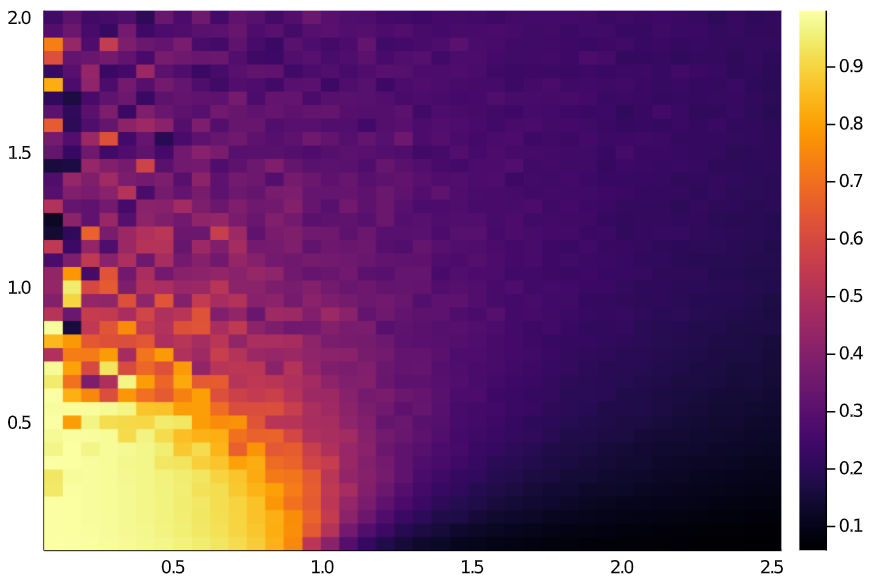
\includegraphics[width=\textwidth]{phase/phase-diagram-transverse-ising-metropolis.PNG}
        \subcaption{}
    \end{subfigure}
    \begin{subfigure}{0.45\textwidth}
        \centering
        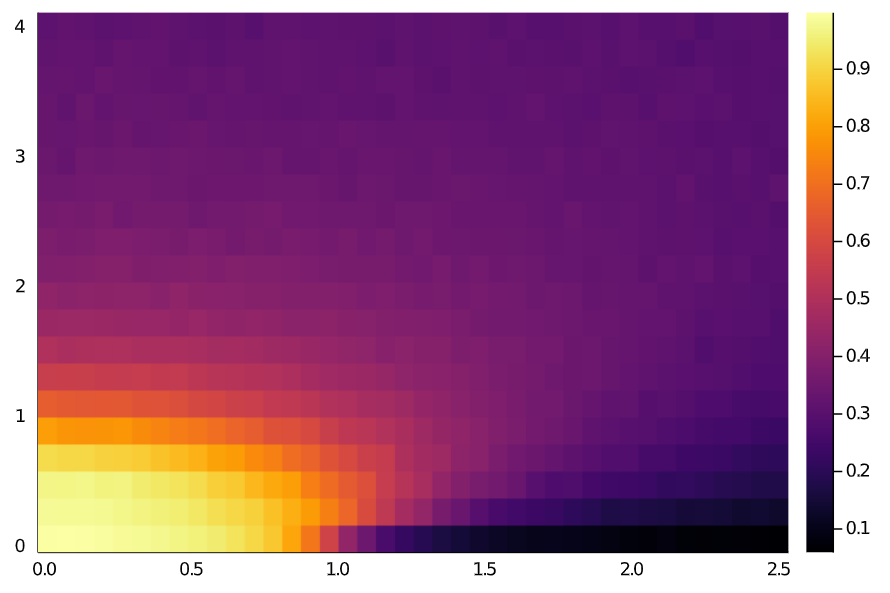
\includegraphics[width=\textwidth]{phase/phase-diagram-transverse-ising-wolff.PNG}
        \subcaption{}
    \end{subfigure}
    \caption{Phase diagrams of 1D transverse field Ising chain obtained with different updating algorithms. The $x$ coordinate is $h$ and the $y$ coordinate is $T$. (a) Metropolis algorithm (b) Wolff cluster algorithm. }
    \label{fig:comparision-metropolis-wolff}
\end{figure}

Since $J_x$ and $J_y$ differ a lot, Metropolis algorithm is incapable for the simulation of the anisotropic Ising model.
Cluster update methods - in this project Wolff cluster updating \cite{Wolff_1989} - must be used.
\autoref{fig:comparision-metropolis-wolff} shows a comparison between Metropolis algorithm and Wolff algorithm, 
where Metropolis algorithm cannot update the system sufficiently when $h=0$, 
since in that case the 2D classical Ising model corresponding to the 1D transverse field Ising chain degenerates into a classical 1D Ising chain due to the vanishing quantum fluctuation, so the coupling strength in the temporal direction approaches to infinite.



\subsection{Get Fermions involved}

\bibliographystyle{plain}
\bibliography{note} 

\end{document}